\section{Double-slit quantum eraser}

\subsection{Case 1: Single photon incident on a double slit apparatus}
\begin{figure}[h!]
    \centering
    \begin{subfigure}{.24\columnwidth}
        \centering
        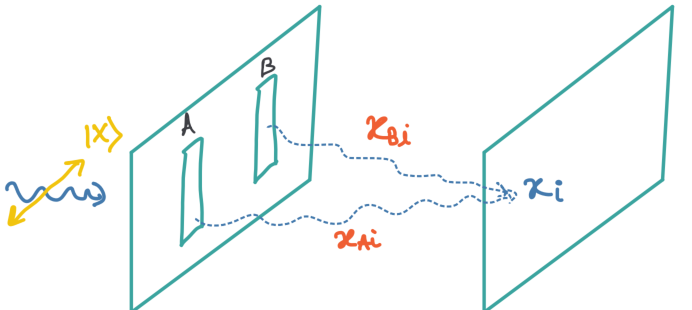
\includegraphics[width=\columnwidth]{PartOne/ChapterThree/figures/doubleslitquantumeraser_case1.png}
        \caption{Case 1}
    \end{subfigure}
    \hfill
    \begin{subfigure}{.24\columnwidth}
        \centering
        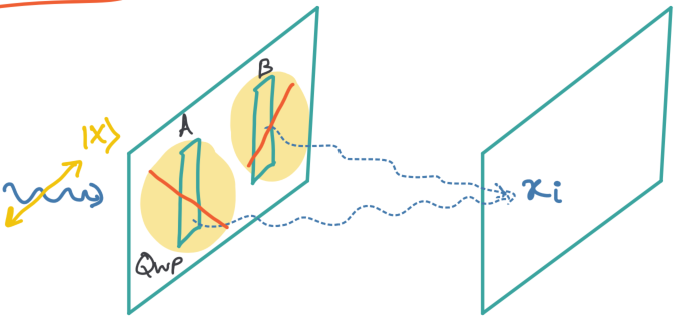
\includegraphics[width=\columnwidth]{PartOne/ChapterThree/figures/doubleslitquantumeraser_case2.png}
        \caption{Case 2}
    \end{subfigure}
    \hfill
    \begin{subfigure}{.24\columnwidth}
        \centering
        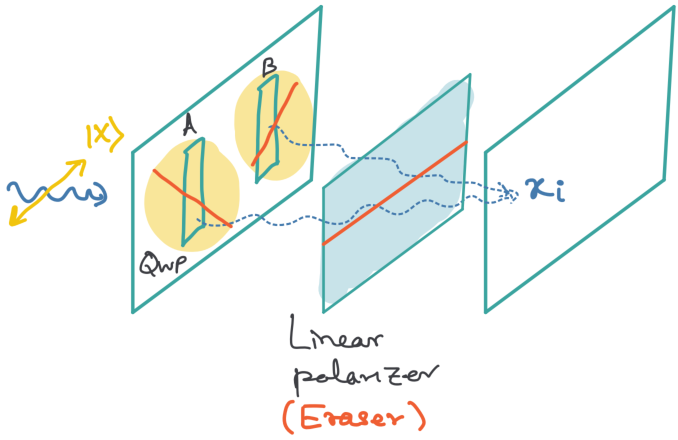
\includegraphics[width=\columnwidth]{PartOne/ChapterThree/figures/doubleslitquantumeraser_case3.png}
        \caption{Case 3}
    \end{subfigure}
    \hfill
    \begin{subfigure}{.24\columnwidth}
        \centering
        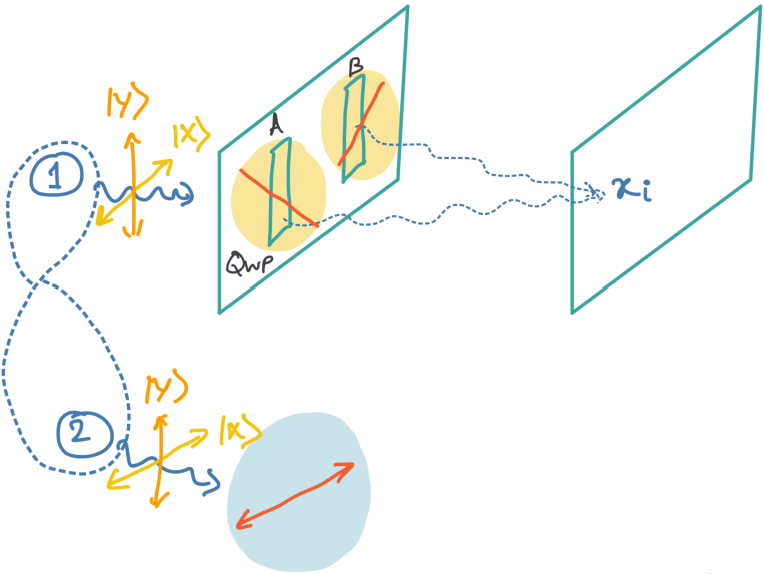
\includegraphics[width=\columnwidth]{PartOne/ChapterThree/figures/doubleslitquantumeraser_case4.png}
        \caption{Case 4}
    \end{subfigure}
    \caption{Double-slit quantum eraser with different cases.}
\end{figure}

The state of the photon after it passes through the slit is:
\begin{align*}
    \ket{\psi}=\frac{1}{\sqrt{2}}\underbrace{(\ket{A}+\ket{B})}_{\text{position}}\otimes\underbrace{\ket{X}}_{\text{polarization}}.
\end{align*}
As the photon propagates from the slit to screen 
\begin{align*}
    \ket{A}\to\sum_i Ne^{ikx_{Ai}}\ket{x_i},\quad\ket{B}\to\sum_iNe^{ikx_{bi}}\ket{x_i}.
\end{align*}
State of the photon at screen is 
\begin{align*}
    \ket{\psi}=\frac{1}{\sqrt{2}}\sum_iN[e^{ikx_{Ai}}+e^{ikx_{Bi}}]\ket{x_i}\otimes\ket{X}=\frac{1}{\sqrt{2}}\sum_iNe^{ikx_{Ai}}[1+e^{ik(x_{Bi}-x_{Ai})}]\ket{x_i}\otimes\ket{X}.
\end{align*}
The probability of finding the photon at psition $x_j$ is:
\begin{align}
    |\braket{x_j|\psi}|^2=\frac{1}{2}|Ne^{ikx_{Ai}}|^2|1+e^{ik(x_{Bj}-x_{Aj})}|^2=2|N|^2\cos^2[\frac{k}{2}(x_{Bj}-x_{Ai})].
\end{align}
%%
\subsection{Case 2: Encoding which path information}
State of the photon after it passes through the two slits is:
\begin{align*}
    \ket{\psi}=\frac{1}{\sqrt{2}}[\ket{A}\ket{+}+\ket{B}\ket{-}],\quad\ket{\pm}=\frac{1}{\sqrt{2}}(\ket{x}\pm i\ket{y}),
\end{align*}
where $\ket{\pm}$ is left and right circularly polarized, respectively.
At the screen:
\begin{align*}
    \ket{\psi}=\frac{1}{\sqrt{2}}\left[\sum_iNe^{ikx_{Ai}}\ket{+}+\sum_iNe^{ikx_{Bi}}\ket{-}\right]\ket{x_i}.
\end{align*}
The probability of detecting a photon at $x_j$ is:
\begin{align*}
    |\braket{x_j|\psi}|^2=\frac{1}{\sqrt{2}}|N|^2|e^{ikx_{Ai}}\ket{+}+e^{ikx_{Bj}}\ket{-}|^2=\frac{2}{\sqrt{2}}|N|^2,\quad\braket{\pm|\mp}=0.
\end{align*}
No interference!
%%
\subsection{Case 3: Erasing which path information}
State after the slit is:
\begin{align*}
    \ket{\psi}=\frac{1}{\sqrt{2}}(\ket{A}\ket{+}+\ket{B}\ket{-}).
\end{align*}
After the eraser:
\begin{align*}
    \ket{\psi}=\frac{1}{\sqrt{2}}\ket{x}\bra{x}(\ket{A}\ket{+}+\ket{B}\ket{-})=\frac{1}{2}(\ket{A}+\ket{B})\otimes\ket{x}.
\end{align*}
Same as case 1 (reduced norm) No which path information. Interference is back!
%%
\subsection{Case 4: Quantum erasure via an entangled photon}
Photon 1 and 2 are entangled in polarization:
\begin{align*}
    \ket{\psi}_{12}=\frac{1}{\sqrt{2}}(\ket{x}_1\ket{x}_2+\ket{y}_1\ket{y}_2).
\end{align*}
After passing through the slits:
\begin{table}[h!]
    \centering
    \begin{tabular}{l|ll}
        &A&B\\
        \hline
        $\ket{x}_1$&$\ket{+}_1$&$\ket{-}_1$\\
        $\ket{y}_2$&$\ket{-}_1$&$\ket{+}_1$
    \end{tabular}
\end{table}

The total state of the photons becomes:
\begin{align*}
    \ket{\psi_{12}}=\frac{1}{2}\left[(\ket{A}_1\ket{+}_1+\ket{B}_1\ket{-}_1)\otimes\ket{x}_2+(\ket{A}_1\ket{-}_1+\ket{B}_1\ket{+}_1)\ket{y}_2\right].
\end{align*}
%%
\subsubsection{Case 4a}
Applying a linear polarizer to photon 2 oriented along x:
\begin{align*}
    \ket{x}_{2}\, {}_{2}\braket{x|\psi_{12}}=\frac{1}{2}(\ket{A}_1\ket{+}_1+\ket{B}_1\ket{-}_1).
\end{align*}
This corresponds to having which-path information (see case 2). No interference. The same if obtained when polarized is oriented along $\ket{y}$.

%%
\subsubsection{Case 4b}
Say the polarizer in photon 2's path is oriented along $\ket{+\pi/4}$:
\begin{align*}
    &\frac{1}{2}(\ket{x}_2+\ket{y}_2)(_2\bra{x}+_2\bra{y})\ket{\psi_{12}}\\
    =&\frac{1}{4}(\ket{x}_2+\ket{y}_2)(_2\bra{x}+_2\bra{y})[(\ket{A}_1\ket{+}_2+
    \ket{B}_1\ket{-}_1)\otimes\ket{x}_2+(\ket{A}_1\ket{-}_1+\ket{B}_1\ket{+}_1)\otimes\ket{y}_2]\\
    =&\frac{1}{2}(\ket{x}_2+\ket{y}_2)[\ket{A}_1\ket{x}_1+\ket{B}_1\ket{x}_1]\\
    =&\frac{1}{2}\underbrace{[\ket{A}_1+\ket{B}_1]}_{\text{No which path!}}\ket{x}_1\otimes(\ket{x}_2+\ket{y}_2).
\end{align*}
Interference is back. Quantum erasure via an entangled photon!